안녕하신가! 힘세고 강한 아침, 만일 내게 물어보면 
나는 영도

근성은 매일 개발 문서를 읽으며 하루를 보낸다.
한국어 문서를 다 읽은 근성은 해외 문서를 읽기 시작했지만, 세상의 다양한 언어로 작성된 개발 문서를 보고 눈앞이 아득해지기 시작했다.
이를 본 영도는 근성을 도와주고자 $N$개 국어 사이의 번역을 일부 제공하는 '정영도봇'(이하 봇) 을 만들었다.

\begin{center}
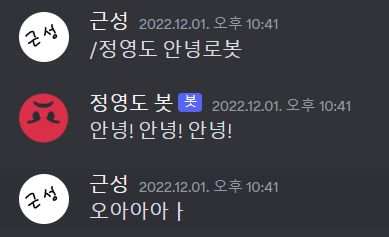
\includegraphics[scale=1]{1.png}
\end{center}

봇은 프로토타입이기에 특이한 번역 로직을 지니고 있다.

\begin{itemize}
 \item 봇은 $N$개의 언어에 대한 데이터를 가지고 있고, 각 언어는 $1$ 이상 $N$ 이하의 중복되지 않는 고유 번호를 가진다. $( 3 \le N \le 100 )$
 \item 번역은 임의의 $A$번 언어 문구를 $B$번 언어 문구로 변환하는 과정을 의미한다.
 \item 번역 시에는 비용이 든다.
 \item 프로토타입이기에 일부 언어 사이에는 번역이 불가능할 수 있다.
 

\end{itemize}
근성은 봇의 성능을 테스트하기 위해 $S$번 언어 문구가 있을 때 특정 $K$번 언어를 거치지 않고 $E$번 언어 문구로 가는 번역 경로가 있는지, 있다면 번역의 그 최소 비용은 얼마인지 여러 번 물어보기 시작했다.

근성의 질문에 답하기 위해 입력값을 하나하나 집어넣던 영도는 진절머리가 나 버렸다.

영도를 위해 봇의 번역 가능성을 판단하는 프로그램을 만들어주자
